\documentclass[sigconf, nonacm]{webmedia}

\usepackage[brazil]{babel}

\AtBeginDocument{%
  \providecommand\BibTeX{{%
    \normalfont B\kern-0.5em{\scshape i\kern-0.25em b}\kern-0.8em\TeX}}}

\settopmatter{printacmref=false, printfolios=false}

\begin{document}

\title{Analisando Grafos do SNAP: o grafo web-flickr (G114)}

\author{Augusto Cesar Ferreira de Quadros}
\email{augustoquadros@ufba.br}
\affiliation{%
  \institution{Universidade Federal da Bahia, Instituto de Computação}
  \city{Salvador}
  \state{BA}
  \country{Brasil}
}

\renewcommand{\shortauthors}{Quadros}

\begin{abstract}
  Este trabalho analisa o web-flickr, grafo da coleção SNAP em que cada vértice é uma imagem do Flickr e cada aresta liga duas imagens que compartilham metadados. A lista de arestas foi convertida em um grafo simples não direcionado, e sobre ele e a sua maior componente conexa calcularam-se, de forma exata, as medidas estruturais pedidas, que reproduzem as estatísticas declaradas pelo SNAP. Os algoritmos de busca em largura e em profundidade, verificação de Eulerianidade, Tarjan, Dijkstra, Bellman-Ford, Floyd-Warshall e Kruskal foram implementados, validados contra o networkx e cronometrados com intervalos de confiança, e os tempos observados foram comparados à complexidade teórica. O grafo apresenta indícios de small-world, com clusterização muito maior que a do grafo aleatório equivalente e comprimento médio dos caminhos próximo do dele. A lei de potência descreve só o extremo da cauda da distribuição de graus. A maior componente resiste à remoção aleatória de 5\% dos vértices e à remoção dos 5\% de maior grau, embora o ataque direcionado isole muito mais vértices da periferia. A descoberta mais interessante é que os vértices de maior grau ficam em grupos densos e redundantes entre si, e não são os elos que mantêm a rede conectada.

\end{abstract}

\keywords{teoria dos grafos, SNAP, web-flickr, análise de redes}

\maketitle

\section{Determinação do grafo}
\label{sec:determinacao}

O grafo analisado é determinado pelo número de matrícula $M$, segundo a regra
\begin{equation}
  f(M) = \big(s(M) \times (u(M) + 1)\big) \bmod 129,
\end{equation}
em que $s(M)$ é a soma dos dígitos de $M$ e $u(M)$ é o número formado pelos dois últimos dígitos de $M$. Se o resultado for $0$, considera-se $129$. O valor obtido é o índice do grafo na planilha ANALISANDO-SNAP-DATASET, que lista os grafos G1 a G129.

Para a matrícula $M = 224215938$:
\begin{align*}
  s(M) &= 2 + 2 + 4 + 2 + 1 + 5 + 9 + 3 + 8 = 36,\\
  u(M) &= 38,\\
  s(M) \times (u(M) + 1) &= 36 \times 39 = 1404,\\
  1404 \bmod 129 &= 1404 - 10 \times 129 = 1404 - 1290 = 114.
\end{align*}

Logo, $f(224215938) = 114$, e o grafo atribuído é o G114 da planilha: o web-flickr, da coleção do SNAP~\cite{snapnets}.

\section{Descrição do grafo original}
\label{sec:descricao}

O web-flickr faz parte da coleção de grafos do SNAP (Stanford Large Network Dataset Collection)~\cite{snapnets} e foi construído por McAuley e Leskovec~\cite{mcauley2012image} para estudar a rotulação de imagens com o uso de metadados de redes sociais.

Cada vértice é uma imagem do Flickr. Uma aresta liga duas imagens que compartilham metadados: imagens do mesmo local, submetidas à mesma galeria, grupo ou conjunto, com tags em comum, do mesmo usuário ou tiradas por amigos. A relação é simétrica, então o grafo é não direcionado. O SNAP distribui o grafo como uma lista de arestas comprimida, \texttt{flickrEdges.txt.gz}, em que cada par não ordenado de vértices aparece uma vez. Além dela, o SNAP distribui atributos dos vértices, atributos das arestas e os metadados das imagens em XML. Este trabalho usa só a lista de arestas, e a Seção~\ref{sec:discussao} explica por que os atributos das arestas não foram usados como pesos.

O SNAP declara as seguintes estatísticas para o grafo~\cite{snapnets}: 105.938 vértices, 2.316.948 arestas, maior componente conexa com 105.722 vértices, coeficiente de clusterização médio de 0,0891, 107.987.357 triângulos e diâmetro 9. Esses valores servem apenas de referência: o tratamento dos dados é descrito na Seção~\ref{sec:tratamento}, e as medidas são recalculadas a partir do arquivo original na Seção~\ref{sec:parte1}.

\subsection{Tratamento realizado}
\label{sec:tratamento}

O arquivo original foi convertido em um grafo simples não direcionado, e dele se extraiu a maior componente conexa. A Tabela~\ref{tab:tratamento} compara os três conjuntos.

\begin{table}[htbp]
  \centering
  \caption{Vértices, arestas, auto-laços e arestas repetidas da lista de arestas original, do grafo simples obtido pelo tratamento e da sua maior componente conexa.}
  \label{tab:tratamento}
  \begin{tabular}{lrrr}
\toprule
 & Lista bruta & Grafo simples & Maior componente \\
\midrule
Vértices & 105.938 & 105.938 & 105.722 \\
Arestas & 2.316.948 & 2.316.948 & 2.316.668 \\
Auto-laços & 0 & 0 & 0 \\
Arestas repetidas & 0 & 0 & 0 \\
\bottomrule
\end{tabular}

\end{table}

Cada linha do arquivo foi tratada como uma aresta não ordenada, porque a relação entre imagens que compartilham metadados é simétrica. Os auto-laços foram removidos e, entre as arestas que ligam o mesmo par de vértices, em qualquer ordem, manteve-se uma só, de modo que o resultado é um grafo simples. A Tabela~\ref{tab:tratamento} mostra que o arquivo original não tinha auto-laços nem arestas repetidas, o que confirma a declaração do SNAP de que cada par aparece uma vez: o grafo simples tem os mesmos vértices e arestas da lista original. O conjunto de vértices é o dos extremos das arestas, pois o arquivo não lista vértices isolados.

Os vértices foram renumerados de $0$ a $n-1$, na ordem crescente do identificador original, para que possam indexar diretamente as listas de adjacência usadas pelas implementações. O identificador original de cada vértice foi guardado em um mapa, que permite voltar às imagens do Flickr.

O grafo é desconexo: a maior componente conexa não contém todos os vértices (Tabela~\ref{tab:tratamento}). O seu tamanho coincide com os 105.722 vértices declarados pelo SNAP. A maior componente recebeu numeração própria, de $0$ a $n_{\mathrm{lcc}}-1$, também registrada no mapa de identificadores.

A política adotada para o grafo desconexo foi a seguinte:
\begin{itemize}
  \item O grafo simples completo é usado nas medidas que não dependem de conexidade (número de vértices e de arestas, graus e sua distribuição, densidade, componentes conexas, coeficiente de clusterização e triângulos) e nos algoritmos que se aplicam a grafos desconexos (busca em largura e em profundidade, verificação de eulerianidade, pontos de articulação e pontes, Dijkstra).
  \item A maior componente conexa é usada nas medidas de distância (diâmetro, raio, comprimento médio dos caminhos e o comprimento médio da análise small-world), porque a distância entre vértices de componentes diferentes é infinita. Ela também é usada na árvore geradora mínima, porque só um grafo conexo tem árvore geradora, e na análise de robustez, como recomenda a descrição do trabalho.
\end{itemize}
Como a maior componente reúne quase todos os vértices e arestas do grafo (Tabela~\ref{tab:tratamento}), as análises feitas sobre ela representam o grafo quase inteiro.

\section{Metodologia}
\label{sec:metodologia}

\subsection{Cálculo das distâncias}

O diâmetro, o raio e o comprimento médio dos caminhos dependem da distância entre todos os pares de vértices da maior componente. Como o grafo não tem pesos, a distância a partir de uma fonte é obtida por uma busca em largura (BFS), em tempo $O(n + m)$, e todas as distâncias, por uma BFS a partir de cada vértice, em tempo $O(n(n + m))$. Optou-se pelo cálculo exato em vez da estimativa por uma amostra de fontes, porque o tempo da passagem completa, executada uma única vez com o igraph, é viável (Tabela~\ref{tab:distancias}). Cada BFS guarda só a excentricidade da fonte e a soma das suas distâncias, e as fontes são processadas em lotes de 500, de modo que a matriz de distâncias, com $n^2$ entradas, nunca fica inteira na memória.

\section{Resultados obtidos}
\label{sec:resultados}

\subsection{Parte I -- Análise estrutural}
\label{sec:parte1}

\subsubsection{Medidas básicas e componentes conexas}

As medidas desta subseção foram calculadas de forma exata sobre o grafo simples completo, com $n$ vértices e $m$ arestas. O grau médio é a média dos graus de todos os vértices, e a densidade é $2m/(n(n-1))$, a fração dos pares de vértices que são ligados por uma aresta. A Tabela~\ref{tab:basicas} reúne os valores.

\begin{table}[htbp]
  \centering
  \caption{Medidas básicas do grafo simples completo, calculadas de forma exata com o networkx.}
  \label{tab:basicas}
  \begin{tabular}{lr}
\toprule
 & Valor \\
\midrule
Vértices ($n$) & 105.938 \\
Arestas ($m$) & 2.316.948 \\
Grau mínimo & 1 \\
Grau máximo & 5.425 \\
Grau médio & 43,741585 \\
Densidade & 0,000413 \\
Componentes conexas & 83 \\
\bottomrule
\end{tabular}

\end{table}

Os números de vértices e de arestas coincidem com os declarados pelo SNAP~\cite{snapnets}, como esperado, já que o tratamento não removeu nenhuma aresta (Seção~\ref{sec:tratamento}). O grau médio coincide com $2m/n$, o que confere a soma dos graus com o dobro do número de arestas. O grau mínimo é 1, pois o arquivo só lista vértices que são extremo de alguma aresta. O grau máximo é muito maior que o grau médio, ou seja, há vértices com muito mais vizinhos que o típico. A densidade é inferior a um milésimo: apesar de cada imagem ter, em média, dezenas de vizinhas, o grafo é esparso, porque o número de pares possíveis cresce com $n^2$ e o de arestas não acompanha esse crescimento.

O grafo tem várias componentes conexas (Tabela~\ref{tab:basicas}). Como a maioria delas é muito pequena, a Tabela~\ref{tab:componentes} não lista cada componente: a maior aparece sozinha na primeira linha, e as demais são agrupadas por tamanho, com o número de componentes de cada tamanho. O número de componentes obtido pelo networkx foi conferido com o do igraph, e a soma dos tamanhos de todas as componentes é igual a $n$.

\begin{table}[htbp]
  \centering
  \caption{Componentes conexas do grafo simples completo agrupadas por tamanho (número de vértices): para cada tamanho, o número de componentes que o têm.}
  \label{tab:componentes}
  \begin{tabular}{rr}
\toprule
Tamanho & Componentes \\
\midrule
105.722 & 1 \\
11 & 1 \\
10 & 1 \\
8 & 1 \\
6 & 1 \\
5 & 2 \\
4 & 3 \\
3 & 13 \\
2 & 60 \\
\bottomrule
\end{tabular}

\end{table}

A Tabela~\ref{tab:componentes} mostra uma componente gigante, cujo tamanho coincide com os 105.722 vértices declarados pelo SNAP~\cite{snapnets}, e uma coleção de componentes minúsculas, a maior delas com 11 vértices e a maioria formada por pares de imagens ligadas só entre si. Essas componentes são grupos de imagens que não compartilham metadados com o restante da coleção. Como reúnem uma parcela desprezível dos vértices, a política de usar a maior componente nas medidas de distância (Seção~\ref{sec:tratamento}) praticamente não descarta informação.

\subsubsection{Distribuição de graus}

A distribuição de graus foi calculada de forma exata sobre o grafo simples completo: para cada grau $k$, contou-se o número de vértices com esse grau, e $P(k)$ é essa contagem dividida por $n$. A soma das contagens é igual a $n$, e a soma de $k$ vezes a contagem de cada grau é igual a $2m$, como deve ser.

\begin{figure}[htbp]
  \centering
  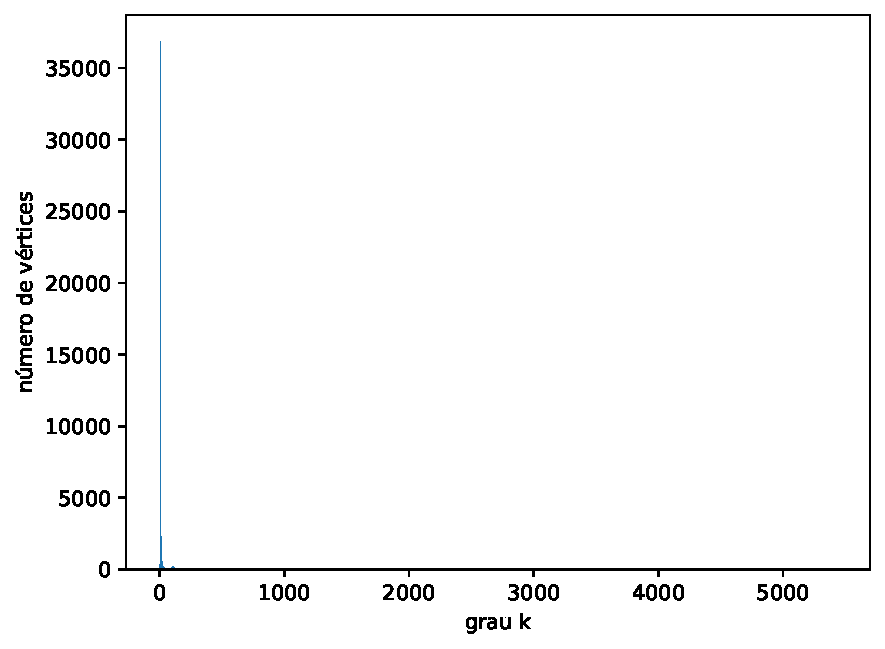
\includegraphics[width=\columnwidth]{../results/figures/graus_hist.pdf}
  \caption{Histograma dos graus do grafo simples completo em escala linear: para cada grau $k$, o número de vértices que o têm.}
  \label{fig:graus_hist}
\end{figure}

Na escala linear (Figura~\ref{fig:graus_hist}), quase toda a massa da distribuição se concentra numa barra estreita junto da origem, enquanto o eixo horizontal se estende até o grau máximo da Tabela~\ref{tab:basicas}. A distribuição é, portanto, fortemente assimétrica à direita: a maioria das imagens tem poucas vizinhas, e uns poucos vértices de grau muito alto, invisíveis nessa escala, puxam o grau médio para bem acima do grau típico.

\begin{figure}[htbp]
  \centering
  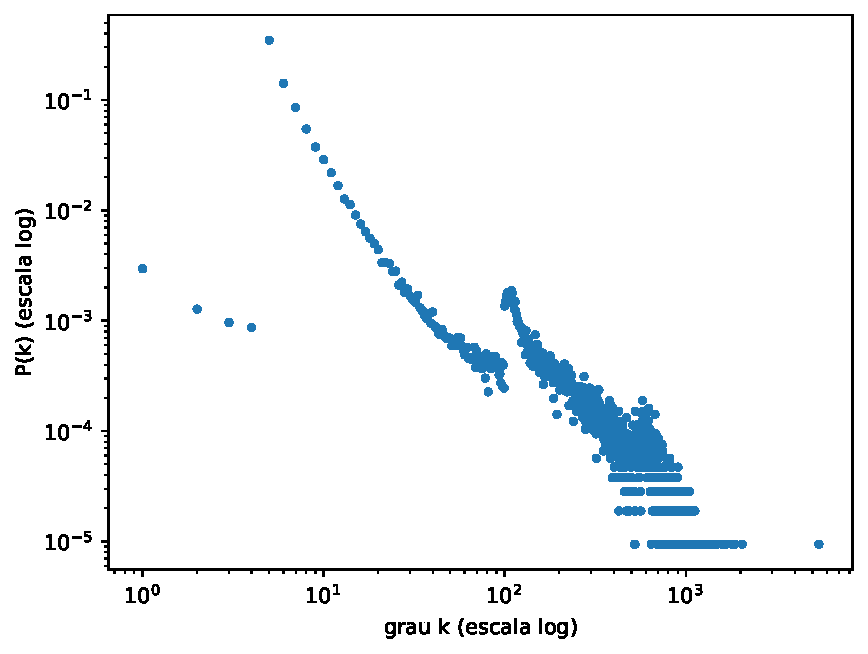
\includegraphics[width=\columnwidth]{../results/figures/graus_loglog.pdf}
  \caption{Distribuição de graus $P(k)$ do grafo simples completo em escala log-log: cada ponto é a fração dos vértices com grau $k$.}
  \label{fig:graus_loglog}
\end{figure}

A escala log-log (Figura~\ref{fig:graus_loglog}) revela o que a escala linear esconde. Os graus de 1 a 4 são raros, e o valor mais frequente é $k = 5$. A partir dele, $P(k)$ decresce de forma contínua ao longo de mais de duas ordens de grandeza de $k$, com uma elevação local perto de $k = 100$. A cauda é longa: há vértices com centenas e milhares de vizinhos, os hubs do grafo, e o de maior grau fica isolado no extremo direito, bem distante dos demais. Na cauda, muitos graus aparecem uma única vez, o que forma a faixa horizontal de pontos na base da figura. Se essa cauda segue ou não uma lei de potência é examinado na Seção~\ref{sec:parte3}.

\subsection{Parte II -- Algoritmos}
\label{sec:parte2}

\subsection{Parte III -- Perguntas}
\label{sec:parte3}


\section{Discussão crítica}
\label{sec:discussao}

Esta seção discute as limitações das decisões tomadas ao longo do trabalho e o quanto cada uma afeta os resultados.

\paragraph{Tratamento dos dados.} O grafo foi reduzido à lista de arestas, sem pesos e sem distinção entre os critérios de ligação (Seção~\ref{sec:tratamento}). Uma aresta entre imagens do mesmo local vale o mesmo que uma entre imagens com uma tag em comum, e um par que compartilha vários metadados vale o mesmo que um que compartilha um só. As medidas descrevem, portanto, a união de relações diferentes, e não permitem dizer qual critério produz a clusterização alta ou os hubs. Além disso, o arquivo só lista imagens com pelo menos uma aresta (Tabela~\ref{tab:basicas}), de modo que as imagens sem metadados em comum com nenhuma outra não fazem parte de $n$. As medidas de distância e a robustez usam só a maior componente, mas essa restrição pesa pouco, porque ela reúne quase todos os vértices e arestas (Tabela~\ref{tab:tratamento}).

\paragraph{Estimativas por amostragem.} Quase todas as medidas da Parte I são exatas (Tabela~\ref{tab:cobertura_parte1}). São estimados o comprimento médio da análise small-world, a partir de 1.000 fontes, e a métrica C da robustez, a partir de 100 fontes. No primeiro caso, o valor exato da Tabela~\ref{tab:distancias} está dentro do intervalo de confiança da Tabela~\ref{tab:small_world}, e a amostragem não afeta a conclusão. No segundo, a estimativa da maior componente original difere do valor exato só nos centésimos (Tabelas~\ref{tab:distancias} e~\ref{tab:robustez_comparacao}), bem menos que a diferença entre os cenários aleatório e direcionado. O cenário direcionado, porém, é uma única execução, sem medida de dispersão, e o desvio do cenário aleatório mistura a variação dos vértices removidos com a das fontes sorteadas. A visualização (Figura~\ref{fig:visualizacao}) é uma amostra parcial e só ilustra a estrutura local.

\paragraph{Política de pesos artificiais.} Como o grafo não tem pesos, os algoritmos de caminhos mínimos e de árvore geradora mínima usaram pesos inteiros sorteados uniformemente em $[1, 10]$ com semente fixa (Seção~\ref{sec:parte2}). Esses pesos não carregam informação sobre as imagens: as distâncias e o peso da árvore das Tabelas~\ref{tab:tempos_caminhos}, \ref{tab:tempos_floyd} e~\ref{tab:tempos_agm} são propriedades do sorteio, e não do grafo, e servem apenas para exercitar e validar os algoritmos. Também os tempos dependem dos pesos: o número de rodadas do Bellman-Ford é limitado pelo número de arestas dos caminhos mínimos, que muda com os pesos.

Os atributos de aresta que o SNAP distribui em \texttt{edgeFeaturesFlickr.tar.gz} não servem de peso. Cada par de imagens tem um vetor de atributos, com contagens de metadados em comum e indicadores, sem uma escala única, e reduzi-lo a um número exigiria uma combinação arbitrária. Os arquivos são separados pela coleção de origem das imagens (CLEF, MIR, PASCAL e NUS). Só parte das arestas de \texttt{flickrEdges.txt.gz} tem atributos, de modo que as demais ficariam sem peso, e a maioria dos pares com atributos não é aresta do grafo. Os pesos $w_{ij}$ do artigo de origem~\cite{mcauley2012image} também não servem: são potenciais aprendidos para cada categoria de rótulo, e não um peso por aresta.

\paragraph{Tempos medidos em uma única máquina.} Todas as medições foram feitas numa única máquina (Seção~\ref{sec:metodologia}). Os valores absolutos dependem do processador, da memória, do sistema operacional e das versões do Python e das bibliotecas, e mudariam em outra máquina. O intervalo de confiança cobre só a variação entre as repetições nessa máquina, e não entre máquinas. O que se transfere é a tendência de crescimento com o tamanho da entrada, comparada à complexidade teórica. Mesmo ela é afetada pela máquina: a hierarquia de memória é uma explicação compatível com a inclinação do Floyd-Warshall acima de 3 (Figura~\ref{fig:floyd_escala}), sem ter sido medida, e a interferência de outros processos é uma explicação possível para os desvios maiores de algumas entradas (Tabela~\ref{tab:tempos_buscas}). As comparações entre o networkx e o igraph (Tabela~\ref{tab:clusterizacao}) refletem sobretudo a linguagem de cada implementação, Python ou C, e não o algoritmo. Por fim, os subgrafos crescentes são aninhados e não crescem de forma uniforme em $m$, e cinco pontos por algoritmo dão uma tendência, não uma estimativa precisa da ordem de crescimento.

\paragraph{Interpretação de small-world.} As referências aleatórias preservam só $n$ e o grau médio, e não a distribuição de graus, fortemente assimétrica (Figura~\ref{fig:graus_loglog}). Uma referência que preservasse também os graus de cada vértice não foi avaliada, e os seus valores de $C_{\mathrm{rand}}$ e $L_{\mathrm{rand}}$ poderiam ser outros. Além disso, $C_{\mathrm{rand}} \approx \langle k \rangle/n$ diminui quando $n$ cresce com $\langle k \rangle$ fixo, de modo que $C/C_{\mathrm{rand}}$ e $\sigma$ tendem a ser grandes em qualquer grafo grande e esparso com clusterização apreciável. A magnitude de $\sigma$ (Tabela~\ref{tab:small_world}) reflete, em parte, o tamanho do grafo. A conclusão se apoia mais na comparação direta de $C$ e de $L$ com as referências. Por fim, a clusterização alta pode ser, em parte, consequência da própria regra de construção, que liga entre si as imagens que compartilham um metadado (Seção~\ref{sec:descricao}), e não uma propriedade que emerge da rede.

\paragraph{Interpretação da lei de potência.} As limitações do ajuste foram discutidas junto da resposta (Seção~\ref{sec:parte3}): o trecho ajustado cobre menos de uma década de $k$ e uma pequena fração dos vértices (Tabela~\ref{tab:lei_potencia}), não há teste de hipótese nem comparação com distribuições alternativas, e o estimador de $\alpha$ é aproximado. A elevação local da distribuição perto de $k = 100$ (Figura~\ref{fig:graus_loglog}) mostra, além disso, que a distribuição tem estrutura que nenhuma lei de potência única descreve. O resultado não permite, portanto, classificar o grafo como livre de escala.

\paragraph{Robustez.} A análise usou uma única fração de remoção, 5\%, e, no ataque direcionado, o ranking de grau calculado uma única vez, antes de qualquer remoção (Seção~\ref{sec:parte3}). Um ataque que recalcula o grau após cada remoção e ataques por outras centralidades, como a betweenness, evitada pelo custo, não foram avaliados. A conclusão de que a rede não é muito mais vulnerável ao ataque direcionado vale, portanto, para esse ataque e essa fração, pelo critério de $S$ e do comprimento médio. Pelas métricas B e D, o ataque fragmenta a periferia muito mais que a falha aleatória (Tabela~\ref{tab:robustez_comparacao}).

\section{Conclusão}
\label{sec:conclusao}

Este trabalho aplicou os conceitos da disciplina ao web-flickr, o grafo G114, em que as imagens do Flickr são ligadas por metadados compartilhados: tratou a lista de arestas, mediu a estrutura do grafo, implementou e cronometrou os algoritmos estudados e respondeu às perguntas obrigatórias sobre a sua estrutura.

O tratamento mostrou que a lista de arestas já formava um grafo simples (Tabela~\ref{tab:tratamento}), e as medidas exatas da Parte I reproduziram os valores declarados pelo SNAP para os vértices, as arestas, a maior componente, os triângulos, o coeficiente de clusterização médio e o diâmetro (Tabelas~\ref{tab:basicas}, \ref{tab:clusterizacao} e~\ref{tab:distancias}). Na Parte II, as implementações próprias deram os mesmos resultados que o networkx, e os tempos medidos acompanharam a complexidade teórica de cada algoritmo. O Bellman-Ford com parada antecipada ficou muito abaixo do limite $O(nm)$ do pior caso, porque poucas rodadas bastam neste grafo (Tabela~\ref{tab:tempos_caminhos}), e o Floyd-Warshall cresceu com expoente um pouco acima do 3 teórico (Figura~\ref{fig:floyd_escala}).

As respostas às perguntas obrigatórias são as seguintes.
\begin{itemize}
  \item \emph{Small-world}: sim. O coeficiente de clusterização é duas ordens de grandeza maior que o do grafo aleatório equivalente, e o comprimento médio dos caminhos fica próximo do dele, de modo que $\sigma$ fica muito acima de 1 (Tabela~\ref{tab:small_world}). Isso é coerente com um grafo em que cada metadado reúne imagens num grupo denso e cada imagem pertence a vários grupos.
  \item \emph{Lei de potência}: só em parte. O ajuste vale apenas no extremo da cauda, que reúne uma pequena fração dos vértices e menos de uma década de graus (Tabela~\ref{tab:lei_potencia} e Figura~\ref{fig:ccdf_loglog}), e não permite classificar o grafo como livre de escala.
  \item \emph{Robustez}: a rede é robusta à remoção aleatória de 5\% dos vértices, que quase só remove os vértices sorteados (Tabela~\ref{tab:robustez_aleatoria}). Também não é muito mais vulnerável à remoção dos 5\% de maior grau, pelo critério da maior componente e do comprimento médio, mas esse ataque isola muito mais vértices da periferia que a falha aleatória (Tabela~\ref{tab:robustez_comparacao}).
  \item \emph{Descoberta mais interessante}: os vértices de maior grau não são os elos que mantêm a rede conectada. Eles ficam em grupos densos e redundantes entre si, como indicam a transitividade bem maior que o coeficiente médio (Tabela~\ref{tab:clusterizacao}) e o ataque direcionado, que quase não reduz a maior componente e só desliga as imagens ligadas apenas aos hubs (Tabela~\ref{tab:robustez_comparacao}).
\end{itemize}

Essas conclusões valem para a lista de arestas, sem a distinção entre os metadados que geraram cada ligação, e com as limitações discutidas na Seção~\ref{sec:discussao}. Uma referência aleatória que preserve a distribuição de graus, testes de hipótese contra distribuições alternativas à lei de potência e ataques que recalculam a centralidade a cada remoção são os passos que tornariam essas respostas mais firmes.

\section{Repositório}
\label{sec:repositorio}

Os códigos, o notebook, os dados tratados e o README com as instruções de execução estão no repositório \url{https://github.com/Augustocfq/snap-flickr-MATA53}.


\bibliographystyle{ACM-Reference-Format}
\bibliography{referencias}

\end{document}
